\documentclass[11pt]{article}

\usepackage[margin=1in]{geometry}
\usepackage{times}
\usepackage{graphicx}
\usepackage{booktabs}
\usepackage{amsmath}
\usepackage{amssymb}
\usepackage{hyperref}
\usepackage{xcolor}
\usepackage{enumitem}
\usepackage{multirow}
\usepackage{caption}
\usepackage{subcaption}
\usepackage{listings}
\usepackage{microtype}

\hypersetup{
    colorlinks=true,
    linkcolor=blue,
    citecolor=blue,
    urlcolor=blue
}

\title{\textbf{ChargebackOps: A Cost-Asymmetric Multi-Round OpenEnv Benchmark for Training LLM Agents on Merchant Dispute Operations}}

\author{
    Mitudru Dutta \\
    \texttt{https://huggingface.co/spaces/mitudrudutta/ChargeBackOps} \\
    \texttt{https://github.com/MitudruDutta/chargebackops}
}

\date{\today}

\begin{document}

\maketitle

\begin{abstract}
Large language model agents are increasingly evaluated on tool use, planning, and interaction with structured environments. However, many existing benchmarks remain either short-horizon, puzzle-like, browser-centric, or weakly connected to real cost-sensitive operations. We introduce \textbf{ChargebackOps}, an OpenEnv-compatible environment for merchant-side credit-card chargeback operations. The environment models a cost-asymmetric, partially observable, multi-round dispute workflow in which an agent must triage cases, query internal merchant systems, gather and curate evidence, submit representment packets, respond to issuer review, and decide whether escalation to arbitration is positive expected value. ChargebackOps includes typed action and observation spaces, delayed evidence, wave-based arrivals, deterministic issuer review, arbitration with a fixed fee, an 8-dimensional composable rubric, handcrafted and procedurally generated tasks, and adapters for ISO-style and Stripe-style dispute records. We evaluate scripted policies and show a large discrimination gap between naive and stronger operational policies: a naive empty-packet policy scores $0.000$, while an EV-rational heuristic reaches $0.813$ on the headline catalog. We further report a single-T4 SFT+GRPO training study using Qwen2.5-3B-Instruct. Supervised fine-tuning improves the base model from $0.456$ to $0.536$ overall. GRPO exposes a typed-action evaluation failure mode: invalid but parseable actions can trigger competent heuristic fallback and inflate evaluation scores to the heuristic baseline. We present ChargebackOps as both a practical financial-operations agent benchmark and a case study in reward design, invalid-action attribution, and evaluation robustness for typed-action LLM reinforcement learning.
\end{abstract}

\section{Introduction}

A customer disputes a card payment. The merchant has a limited response window. Evidence is scattered across order logs, payment records, shipping scans, support transcripts, refund ledgers, and fraud-risk systems. Some evidence strengthens the merchant's case; other evidence can harm it. If the merchant escalates to arbitration, both sides pay a fixed fee. The optimal decision is not simply to contest or concede, but to reason about deadlines, evidence quality, issuer behavior, and expected value.

This paper introduces \textbf{ChargebackOps}, an OpenEnv environment that turns merchant chargeback operations into a structured LLM-agent benchmark. The environment targets a class of tasks that we believe is underrepresented in current agent research: \emph{cost-sensitive, evidence-driven, multi-round operational decision-making}. Unlike a static classification benchmark, ChargebackOps requires the agent to choose a sequence of typed actions over time. Unlike a pure retrieval benchmark, the agent must decide which evidence to gather, which evidence to attach, and which evidence to omit. Unlike many toy RL environments, the terminal outcome depends on business economics: escalation is rational only when the expected recovery exceeds a fixed arbitration cost.

The central decision-theoretic primitive is:
\begin{equation}
    P(\text{win}) \cdot \text{amount} > 250,
\end{equation}
where $250$ is the fixed arbitration fee. This simple inequality creates a rich family of policies: always conceding, always contesting, and always escalating are all suboptimal in different parts of the task distribution.

Our contributions are:
\begin{enumerate}[leftmargin=*]
    \item We introduce \textbf{ChargebackOps}, a realistic OpenEnv environment for merchant dispute operations with typed actions, partial observability, delayed events, multi-round issuer review, and arbitration economics.
    \item We implement an \textbf{8-dimensional composable rubric} using OpenEnv-style rubric components, including strategy correctness, evidence quality, packet validity, deadline compliance, efficiency, outcome quality, note quality, and escalation ROI.
    \item We provide a \textbf{benchmark discrimination study} over scripted policies, showing that degenerate policies hit known ceilings while an EV-rational heuristic scores substantially higher.
    \item We report a \textbf{single-T4 SFT+GRPO training study} on Qwen2.5-3B-Instruct, including a legitimate SFT improvement and a diagnostic analysis of a GRPO evaluation fallback exploit.
    \item We release the environment as a Hugging Face Space and GitHub repository, with figures, tests, documentation, and reproducibility instructions.
\end{enumerate}

\section{Related Work}

\paragraph{LLM reinforcement learning and GRPO.}
Policy-gradient methods such as PPO \cite{schulman2017ppo} have become central to modern LLM post-training. GRPO, popularized in DeepSeekMath \cite{shao2024deepseekmath}, removes the value model and computes relative advantages within sampled groups. ChargebackOps uses this family of methods through Hugging Face TRL \cite{trl}. Our diagnostic study focuses on GRPO behavior after supervised fine-tuning in a typed-action environment.

\paragraph{RL with verifiable rewards.}
RLVR replaces learned reward models with programmatic verifiers when outcomes are checkable. ChargebackOps follows this spirit: final rewards are produced by a deterministic environment, issuer model, arbitration model, and rubric tree rather than a learned judge. This connects to recent work on verifiable environments and environment-based RL for agents \cite{lambert2024tulu3, rlve2025}.

\paragraph{Agent environments.}
Recent work has introduced environment platforms for embodied, browser, code, and general agent tasks \cite{browsergym, gem2025}. ChargebackOps differs by targeting a financial-operations workflow with cost-asymmetric terminal economics and multi-round adjudication.

\paragraph{Reward hacking and specification gaming.}
Specification gaming is a long-standing failure mode in reinforcement learning \cite{krakovna2020specification,weng2024rewardhacking,skalse2022rewardhacking}. Our GRPO study provides a concrete typed-action instance: invalid but parseable actions can trigger competent fallback in the rollout helper, causing the trained policy to inherit heuristic reward without producing valid work.

\section{Environment Design}

\subsection{Task Setting}

A chargeback case represents a disputed transaction. Each case contains a reason code, amount, deadline, evidence requirements, possible harmful evidence, and an optimal or acceptable strategy. The agent observes a queue of cases and must act within a fixed step budget.

The environment includes six internal merchant systems:
\begin{itemize}[leftmargin=*]
    \item \textbf{orders}: order confirmations, invoices, SKU and customer records.
    \item \textbf{payment}: authorization, capture, AVS/CVV checks, settlement logs.
    \item \textbf{shipping}: tracking, delivery scans, carrier proof, signatures.
    \item \textbf{support}: chat transcripts, complaints, acknowledgements.
    \item \textbf{refunds}: refund ledger and credit status.
    \item \textbf{risk}: device history, fraud scores, prior good-order linkage.
\end{itemize}

Evidence can be helpful, required, neutral, or harmful. This forces evidence curation rather than evidence accumulation.

\subsection{Action Space}

The environment exposes a typed action space. Round-1 representment actions are:
\begin{center}
\texttt{select\_case}, \texttt{inspect\_case}, \texttt{query\_system}, \texttt{retrieve\_policy}, \texttt{add\_evidence}, \texttt{remove\_evidence}, \texttt{set\_strategy}, \texttt{submit\_representment}, \texttt{resolve\_case}.
\end{center}

Round-2 and round-3 actions are:
\begin{center}
\texttt{respond\_to\_pre\_arb}, \texttt{escalate\_to\_arbitration}, \texttt{accept\_arbitration\_loss}.
\end{center}

Long-horizon backlog management additionally includes:
\begin{center}
\texttt{wait\_for\_updates}.
\end{center}

Every action consumes one step. This makes the step budget meaningful: querying another system, fixing a packet, or waiting for delayed evidence all carry opportunity cost.

\subsection{State and Observation}

The environment follows the OpenEnv reset/step/state contract:
\begin{equation}
    \texttt{reset}(\tau) \rightarrow o_0, \quad
    \texttt{step}(a_t) \rightarrow o_{t+1}, \quad
    \texttt{state}() \rightarrow s_t.
\end{equation}

Observations expose the visible case queue, selected case, retrieved evidence, attached evidence, policy guidance, previous action result, step budget, and final grader report when the episode ends. The hidden scenario state includes optimal strategy, full evidence annotations, delayed event queues, and final scoring metadata.

\section{Dispute Lifecycle}

Figure~\ref{fig:architecture} summarizes the environment loop. The agent emits typed actions. The environment updates case progress, reveals evidence, invokes issuer review, applies arbitration, and finally computes rubric scores.

\begin{figure}[h]
\centering
\fbox{\begin{minipage}{0.92\linewidth}
\centering
\vspace{0.2cm}
Agent $\rightarrow$ Typed Action $\rightarrow$ Environment Step $\rightarrow$ Scenario Data $\rightarrow$ Issuer/Arbitration $\rightarrow$ Rubric Score $\rightarrow$ Observation
\vspace{0.2cm}
\end{minipage}}
\caption{High-level ChargebackOps environment loop.}
\label{fig:architecture}
\end{figure}

\subsection{Issuer Review}

After a representment packet is submitted, a scripted issuer computes an evidence-strength score:
\begin{equation}
    S_{evidence} = f(E_{required}, E_{helpful}, E_{harmful}, N, E_{prearb}),
\end{equation}
where $N$ denotes note quality and $E_{prearb}$ denotes additional pre-arbitration evidence.

The round-1 issuer policy is thresholded:
\begin{equation}
\pi_{issuer}^{(1)} =
\begin{cases}
\text{accept}, & S_{evidence} \geq 0.70, \\
\text{request more evidence}, & S_{evidence} \leq 0.40, \\
\text{ambiguity rule}, & \text{otherwise}.
\end{cases}
\end{equation}

In round 2, the acceptance threshold is lower:
\begin{equation}
\pi_{issuer}^{(2)} =
\begin{cases}
\text{accept}, & S_{evidence} \geq 0.60, \\
\text{escalate to arbitration}, & \text{otherwise}.
\end{cases}
\end{equation}

The issuer is deterministic by default to support reproducible evaluation. Optional LLM softening can be used in ambiguity bands, but the default benchmark path is deterministic.

\subsection{Arbitration}

Arbitration is a terminal adjudication step with fixed fees. If the evidence score is strong enough, the merchant wins; if weak enough, the issuer wins; otherwise a deterministic case-ID-based tie-breaker is used.

The merchant P\&L is:
\begin{equation}
\text{P\&L} =
\begin{cases}
\text{amount} - 250, & \text{merchant wins}, \\
-\text{amount} - 250, & \text{issuer wins}.
\end{cases}
\end{equation}

The rational escalation condition is:
\begin{equation}
    P(\text{win}) \cdot \text{amount} > 250.
\end{equation}

\section{Rubric and Reward Design}

ChargebackOps uses an 8-dimensional rubric. Figure~\ref{fig:rubric} shows the rubric weights.

\begin{figure}[h]
\centering
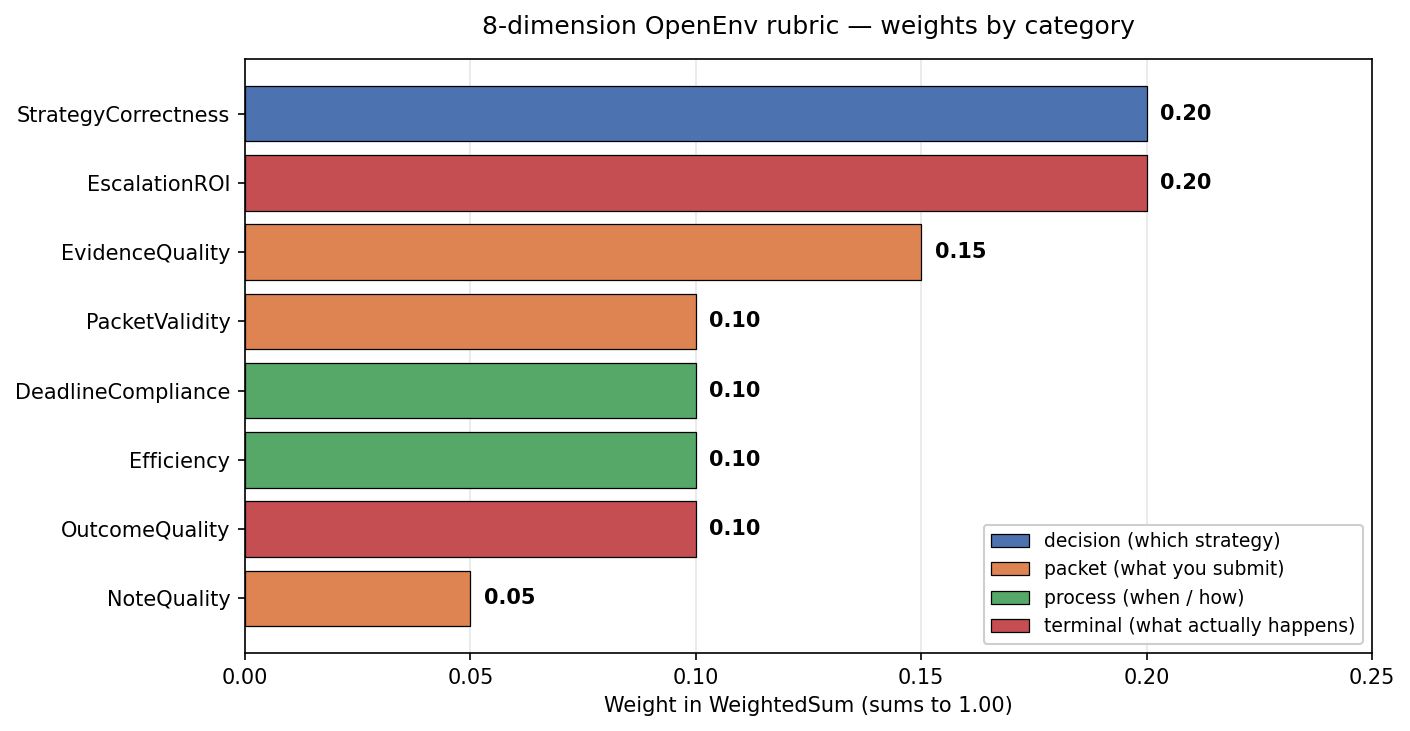
\includegraphics[width=0.92\linewidth]{../docs/figures/rubric_weights.png}
\caption{Eight-dimensional ChargebackOps rubric weights.}
\label{fig:rubric}
\end{figure}

The per-case score is:
\begin{align}
S_{case} ={}& 0.20S_{strategy}
+ 0.15S_{evidence}
+ 0.10S_{packet}
+ 0.10S_{deadline} \\
&+ 0.10S_{efficiency}
+ 0.10S_{outcome}
+ 0.05S_{note}
+ 0.20S_{roi}. \nonumber
\end{align}

A deadline gate hard-zeros abandoned cases:
\begin{equation}
S_{case}^{final} =
\begin{cases}
0, & \text{if abandoned past deadline}, \\
S_{case}, & \text{otherwise}.
\end{cases}
\end{equation}

The episode score is a weighted average over cases:
\begin{equation}
S_{episode} = \frac{\sum_i w_i S_i}{\sum_i w_i}.
\end{equation}

This scoring design is intentionally anti-degenerate. A naive empty-packet policy fails packet validity and deadlines. A concede-all policy receives partial strategy credit on genuinely weak cases but fails positive-EV contests. An escalate-all policy performs strongly on some disputes but loses ROI credit on negative-EV arbitration branches.

\section{Tasks}

ChargebackOps includes handcrafted and generated tasks. Representative tasks include:
\begin{itemize}[leftmargin=*]
    \item \texttt{goods\_not\_received\_easy}: single-case delivery-proof dispute.
    \item \texttt{fraud\_signal\_ambiguity}: fraud case with useful and harmful evidence.
    \item \texttt{queue\_optimization\_hard}: multiple cases with different optimal strategies and deadlines.
    \item \texttt{pre\_arb\_recovery\_medium}: issuer requests additional evidence before final resolution.
    \item \texttt{monthly\_dispute\_backlog\_marathon}: 12 cases, 60 steps, wave arrivals, delayed evidence, delayed issuer responses, and arbitration tradeoffs.
\end{itemize}

The monthly backlog marathon is the flagship long-horizon task. It tests memory, prioritization, pending-work tracking, and portfolio optimization rather than isolated single-case reasoning.

\section{Scripted Policy Benchmark}

We evaluate four scripted policies: naive, concede-all, escalate-all, and heuristic. The results are shown in Table~\ref{tab:baselines} and Figure~\ref{fig:discrimination}.

\begin{table}[h]
\centering
\begin{tabular}{lccc}
\toprule
Policy & Headline Avg & Multi-seed Avg & Description \\
\midrule
naive & 0.000 & 0.000 & Submit empty packet immediately \\
concede\_all & 0.444 & 0.445 & Always accept chargeback \\
escalate\_all & 0.767 & 0.768 & Always contest and escalate \\
heuristic & \textbf{0.813} & 0.763 & EV-rational offline policy \\
\bottomrule
\end{tabular}
\caption{Scripted policy benchmark results.}
\label{tab:baselines}
\end{table}

\begin{figure}[h]
\centering
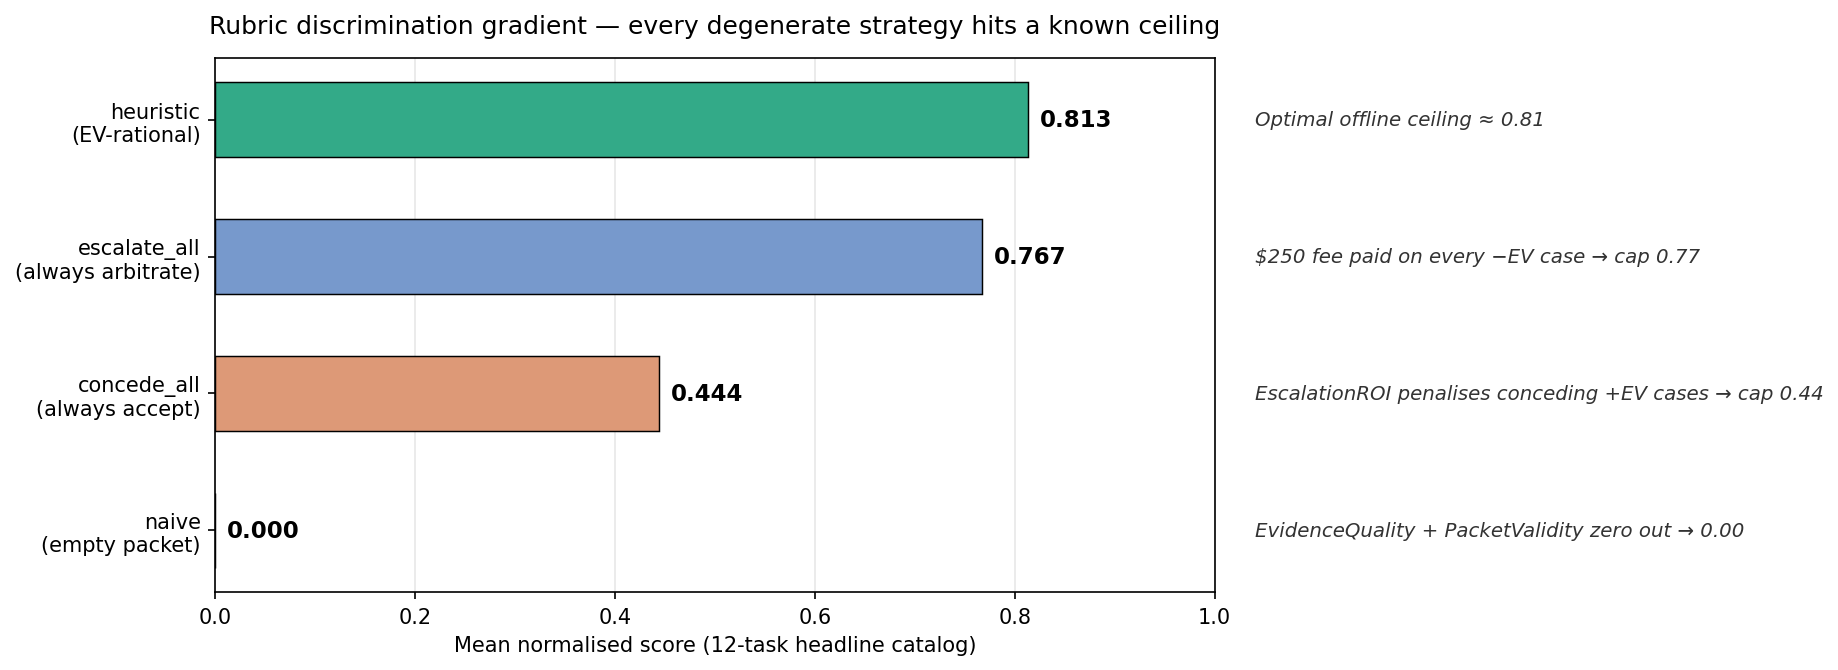
\includegraphics[width=0.92\linewidth]{../docs/figures/discrimination_gradient.png}
\caption{Policy discrimination gradient. Degenerate policies hit known ceilings while the EV-rational heuristic performs best on the headline catalog.}
\label{fig:discrimination}
\end{figure}

The headline discrimination delta is:
\begin{equation}
    \Delta = S_{heuristic} - S_{naive} = 0.813 - 0.000 = 0.813.
\end{equation}

\section{Training Pipeline}

We train Qwen2.5-3B-Instruct with fp16 LoRA on a single T4. The pipeline has two phases.

\paragraph{Phase A: supervised fine-tuning.}
We generate 4,000 prompt/action pairs from heuristic rollouts. The model is fine-tuned with LoRA rank 16 for 150 steps. The goal is to teach the typed action interface and basic workflow behavior.

\paragraph{Phase B: GRPO.}
We use GRPO with an outcome reward and a format reward. The outcome reward normalizes terminal merchant P\&L:
\begin{equation}
    R_{outcome} = \text{normalize}(\text{terminal merchant P\&L}).
\end{equation}

The format reward is:
\begin{equation}
R_{format} =
\begin{cases}
+0.05, & \text{parseable JSON}, \\
-0.10, & \text{unparseable JSON}.
\end{cases}
\end{equation}

The combined reward is:
\begin{equation}
    R = R_{outcome} + R_{format}.
\end{equation}

\section{Training Results}

The clearest legitimate improvement is produced by SFT. The untrained Qwen2.5-3B base scores $0.456$, while the SFT checkpoint scores $0.536$.

\begin{equation}
    \Delta_{SFT} = 0.536 - 0.456 = 0.080.
\end{equation}

The relative improvement is:
\begin{equation}
    \frac{0.536 - 0.456}{0.456} \times 100 \approx 17.54\%.
\end{equation}

\begin{figure}[h]
\centering
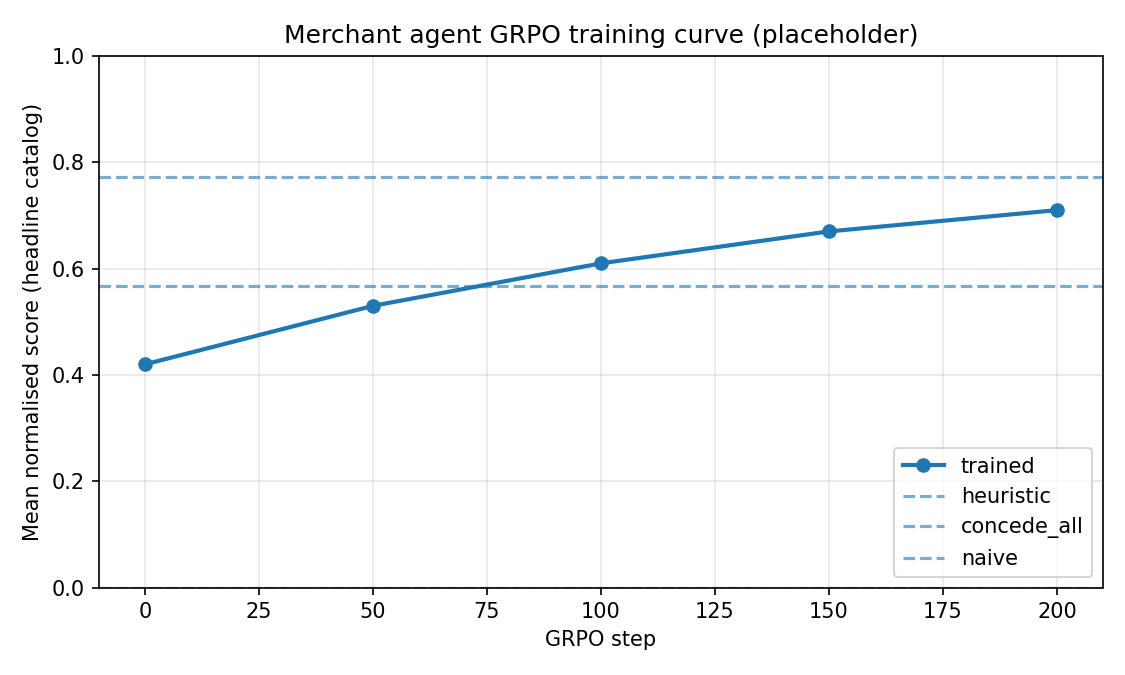
\includegraphics[width=0.92\linewidth]{../docs/figures/training_curve.png}
\caption{Overall training curve. The SFT checkpoint shows legitimate improvement; later GRPO checkpoints require diagnostic attribution due to fallback behavior.}
\label{fig:training}
\end{figure}

\begin{figure}[h]
\centering
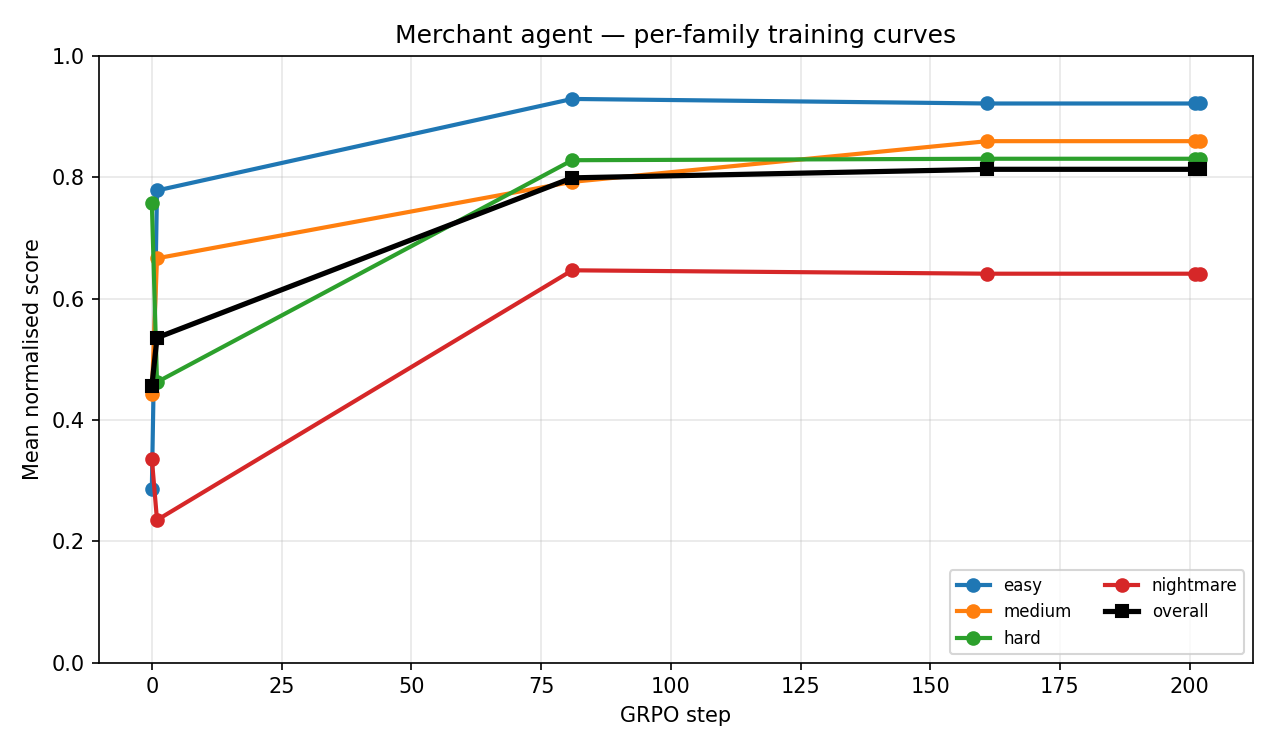
\includegraphics[width=0.92\linewidth]{../docs/figures/training_curve_by_family.png}
\caption{Per-difficulty training behavior. Easy and medium tasks improve more clearly than hard and nightmare tasks.}
\label{fig:family}
\end{figure}

\section{A Typed-Action GRPO Failure Mode}

The GRPO phase revealed a specification-gaming failure mode in the evaluation pipeline. Later checkpoints emitted an invalid but parseable action:
\begin{center}
\texttt{\{"action\_type": "accept\_case", "case\_id": "CB-E1"\}}
\end{center}

The action \texttt{accept\_case} is not valid. The closest valid actions are \texttt{accept\_chargeback}, \texttt{accept\_arbitration\_loss}, and \texttt{select\_case}. Because the rollout helper fell back to a competent heuristic policy on invalid model output, the final score reflected heuristic behavior rather than the trained policy's behavior.

\begin{figure}[h]
\centering
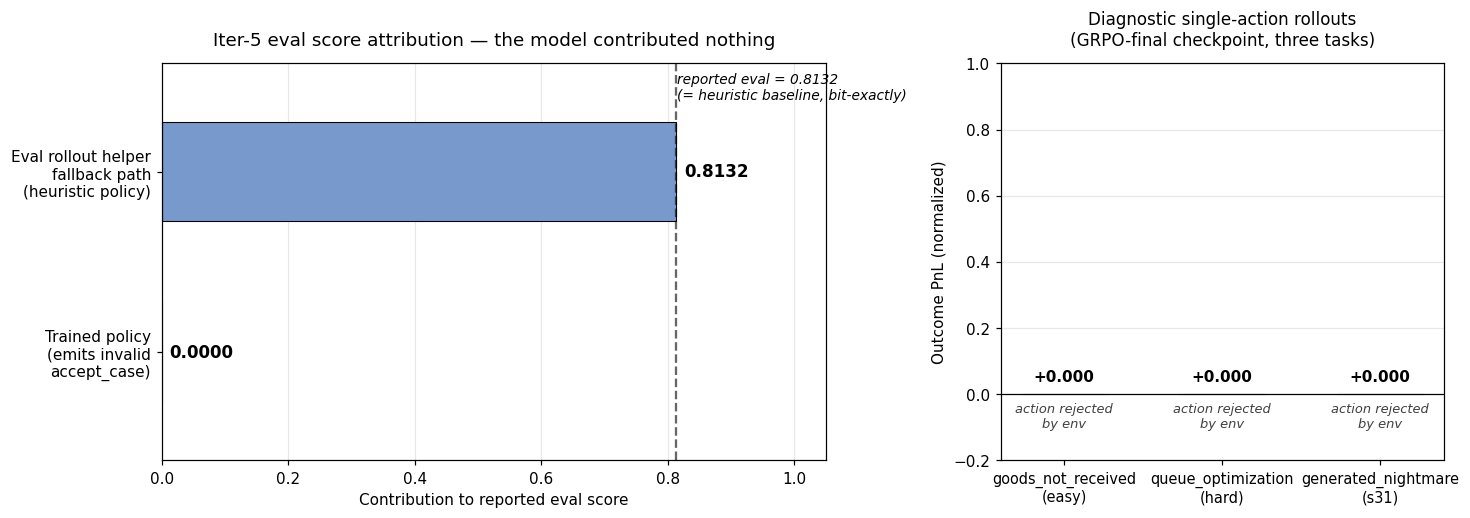
\includegraphics[width=0.92\linewidth]{../docs/figures/gaming_attribution.png}
\caption{Diagnostic attribution: the GRPO-final policy emits invalid actions, while heuristic fallback produces the executed episode behavior.}
\label{fig:gating}
\end{figure}

A corrected evaluation should penalize invalid actions:
\begin{equation}
    S_{eval}^{corrected} = S_{rubric} - \lambda N_{invalid},
\end{equation}
where $\lambda$ is a penalty coefficient and $N_{invalid}$ is the count of invalid model actions.

This failure mode is a useful lesson for typed-action LLM RL: a model should not receive credit for a fallback policy's work.

\section{Limitations}

ChargebackOps is a benchmark and simulation environment, not a production chargeback platform. The issuer is deterministic by default, network rules are simplified relative to full Visa/Mastercard rulebooks, and merchant systems are simulated. These are deliberate design choices to make the environment reproducible, inspectable, and trainable. Future work should add richer network-specific rules, stochastic merchant systems, learned issuer opponents, stricter invalid-action training, and deeper real-data connectors.

\section{Conclusion}

ChargebackOps turns merchant dispute operations into a structured benchmark for long-horizon, cost-sensitive, evidence-driven LLM agents. The environment tests more than document retrieval or summarization: it requires typed actions, partial observability, evidence curation, deadline management, issuer interaction, arbitration economics, and portfolio-level prioritization. Scripted policy results show strong discrimination, and the training study demonstrates both real SFT improvement and a practical GRPO evaluation pitfall. We hope ChargebackOps can serve as a useful environment for researchers studying agentic RL, reward design, verifiable environments, and financially grounded workflow automation.

\bibliographystyle{plain}
\bibliography{references}

\end{document}
